\documentclass[border=8pt]{standalone}
\usepackage{graphicx}
\usepackage{tikz}
\usepackage{xcolor}
\usetikzlibrary{arrows.meta, positioning}
\definecolor{academicblue}{RGB}{30,64,105}
\definecolor{academicgray}{RGB}{100,116,139}
\begin{document}
\resizebox{8.4cm}{!}{%
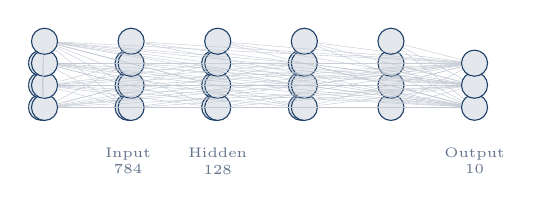
\begin{tikzpicture}[
  font=\scriptsize,
  neuron/.style={circle, draw=academicblue, fill=academicblue!12, minimum size=0.22cm},
  layer label/.style={font=\tiny, text=academicgray, align=center}
]
\def\layersep{1.1cm}
\def\nodesep{0.28cm}
\foreach \i in {1,...,4} {
  \foreach \j in {1,...,3} {
    \node[neuron] (in\i\j) at (\i*\layersep, \j*\nodesep) {};
  }
}
\foreach \i in {1,...,5} {
  \foreach \j in {1,...,4} {
    \node[neuron] (hid\i\j) at (\i*\layersep+1.1, \j*\nodesep-0.05) {};
  }
}
\foreach \j in {1,...,3} {
  \node[neuron] (out\j) at (6.6, \j*\nodesep) {};
}
\foreach \a in {1,...,4} \foreach \b in {1,...,3} \foreach \c in {1,...,4}
  \draw[academicgray!40, line width=0.15pt] (in\a\b) -- (hid1\c);
\foreach \a in {1,...,5} \foreach \b in {1,...,4} \foreach \c in {1,...,3}
  \draw[academicgray!40, line width=0.15pt] (hid\a\b) -- (out\c);
\node[layer label, below=0.5cm of in22] {Input\\784};
\node[layer label, below=0.5cm of hid32] {Hidden\\128};
\node[layer label, below=0.5cm of out2] {Output\\10};
\end{tikzpicture}%
}
\end{document}
